% Asal-usul (tidak pernah dicetak): lihat sources/outline_sources.md (Tahun 1: perpecahan benua;
% tepi pasif; punggungan cepat dan lambat; hukum kedalaman-umur lantai samudra; sesar transform).
% Kurva dari figdata/bachelor-1/depth_age.py; nilai soal latihan dan soal dihitung dalam kalkulator
% skrap Buku 3 calc/ch13.py; koordinat skema tepi dari calc/fig13_margin.py.
\chapter{Celah, punggungan dan tepi pasif}\label{ch:b1:rifts-ridges-margins}

Pada bulan September 2005 tanah di gurun Afar, di timur laut Etiopia, terbuka. Dalam tiga minggu, sepotong celah sepanjang sekitar \qty{60}{km} melebar hingga \qty{8}{m}, dan sekitar \qty{2.5}{km^3} magma naik ke retakan dari bawah. Lempeng-lempeng di sana memisah sekitar \qty{18}{mm} per tahun: krisis itu melepaskan, dalam beberapa minggu, peregangan selama sekitar empat abad. Afar adalah benua yang sedang pecah; beberapa ratus kilometer ke utara, Laut Merah adalah samudra muda yang dasarnya sudah terbentuk seperti dasar Atlantik, dan Atlantik Selatan pernah menjadi celah serupa sebelum terbuka, sekitar 120 juta tahun yang lalu. Bab ini mengikuti kelahiran sebuah samudra: peregangan benua, perpecahannya, dua \omterm{def:b1:rifts-ridges-margins:passive-margin}{tepi pasif} yang tertinggal, punggungan yang membangun dasar samudra, dan penurunan lambat dasar itu ketika ia mendingin.
% ledger: wright:afar, morvel:ar-nb (18.5 mm/yr at 12.3 N, 40.6 E, computed with euler_velocities.py), heine:fit

\begin{recall}
Lempeng adalah \omterm{def:b1:heat-budget:boundary-layer}{lapisan batas termal} atas \omterm{def:b1:layered-earth:layers}{mantel}; di bawah samudra, setengah-ruang yang mendingin menggambarkannya, dan isotermnya menjadi lebih dalam sebanding dengan akar kuadrat umur (\cref{ch:b1:heat-budget}). Kolom batuan dalam kesetimbangan isostatik memiliki massa per satuan luas yang sama di atas \omterm{def:b1:isostasy-gravity:isostasy}{kedalaman kompensasi} (\cref{ch:b1:isostasy-gravity}). Lempeng berputar terhadap \omterm{def:b1:plate-kinematics:euler-pole}{kutub Euler}, punggungan menyebar dengan laju yang dibaca dari anomali magnetik, dan transform terletak pada \omterm{def:b1:spherical-astronomy:spherical-triangle}{lingkaran kecil} terhadap kutub (\cref{ch:b1:plate-kinematics}). Lemparan dan pergeseran horizontal sebuah sesar didefinisikan di \cref{ch:b1:cross-sections}; sesar normal adalah sesar miring yang blok atasnya telah turun (Buku 2, kelas 11).
\end{recall}

\section{Pemekaran benua}

Benua yang diregangkan oleh gaya di tepinya tidak menipis secara merata. \omterm{def:b1:layered-earth:layers}{Kerak} atasnya yang rapuh pecah sepanjang sesar normal, dan blok-blok di antaranya tenggelam dan miring; di bawahnya, \omterm{def:b1:layered-earth:layers}{kerak} bawah yang lebih hangat dan \omterm{def:b1:layered-earth:layers}{mantel} mengalir.

\begin{definition}[Celah benua, graben, paruh-graben]\label{def:b1:rifts-ridges-margins:rift}
Sebuah \emph{celah benua}\index{celah benua} adalah zona panjang dan sempit tempat sebuah benua sedang diregangkan: depresi yang dibatasi sesar normal, disertai gempa bumi dan, sering kali, gunung api. \emph{Graben}\index{graben} adalah blok yang turun di antara dua sesar normal yang masing-masing miring ke arah satu sama lain. \emph{Paruh-graben}\index{paruh-graben} adalah blok yang turun dan miring terhadap satu sesar normal utama, sesar batas, hanya di satu sisi.
\end{definition}

Sebagian besar basin celah adalah rangkaian \omterm{def:b1:rifts-ridges-margins:rift}{paruh-graben}. Sesar-sesar batasnya menyerahkan pergeseran satu sama lain melalui rampa relai, dan sisi tempat sesar batas berada sering berganti dari satu segmen ke segmen berikutnya. Dinding gantung setiap sesar batas miring ke bawah ke arahnya, dan basin paling cepat terisi di sana: sedimen paling tebal menumpuk di sepanjang sesar, sementara dinding bawah terangkat menjadi bahu celah.

Peregangan horizontal yang dibawa sebuah sesar adalah pergeseran horizontalnya. Sesar normal planar dengan lemparan $h$ dan \omterm{def:b1:geological-maps:attitude}{kemiringan} $\delta$ memiliki pergeseran horizontal $h/\tan\delta$ (\cref{ch:b1:cross-sections}); menjumlahkan pergeseran horizontal sesar-sesar di sepanjang penampang celah memberikan perpanjangan \omterm{def:b1:layered-earth:layers}{kerak} rapuh. Bagaimana seluruh \omterm{def:b1:layered-earth:lithosphere}{litosfer} menipis ketika diregangkan, dan mengapa ia kemudian turun, dikuantifikasi dalam volume Tahun ke-2; di sini sesar-sesar diukur, dan jumlahnya dibandingkan dengan gerak
lempeng.

\begin{omfigure}
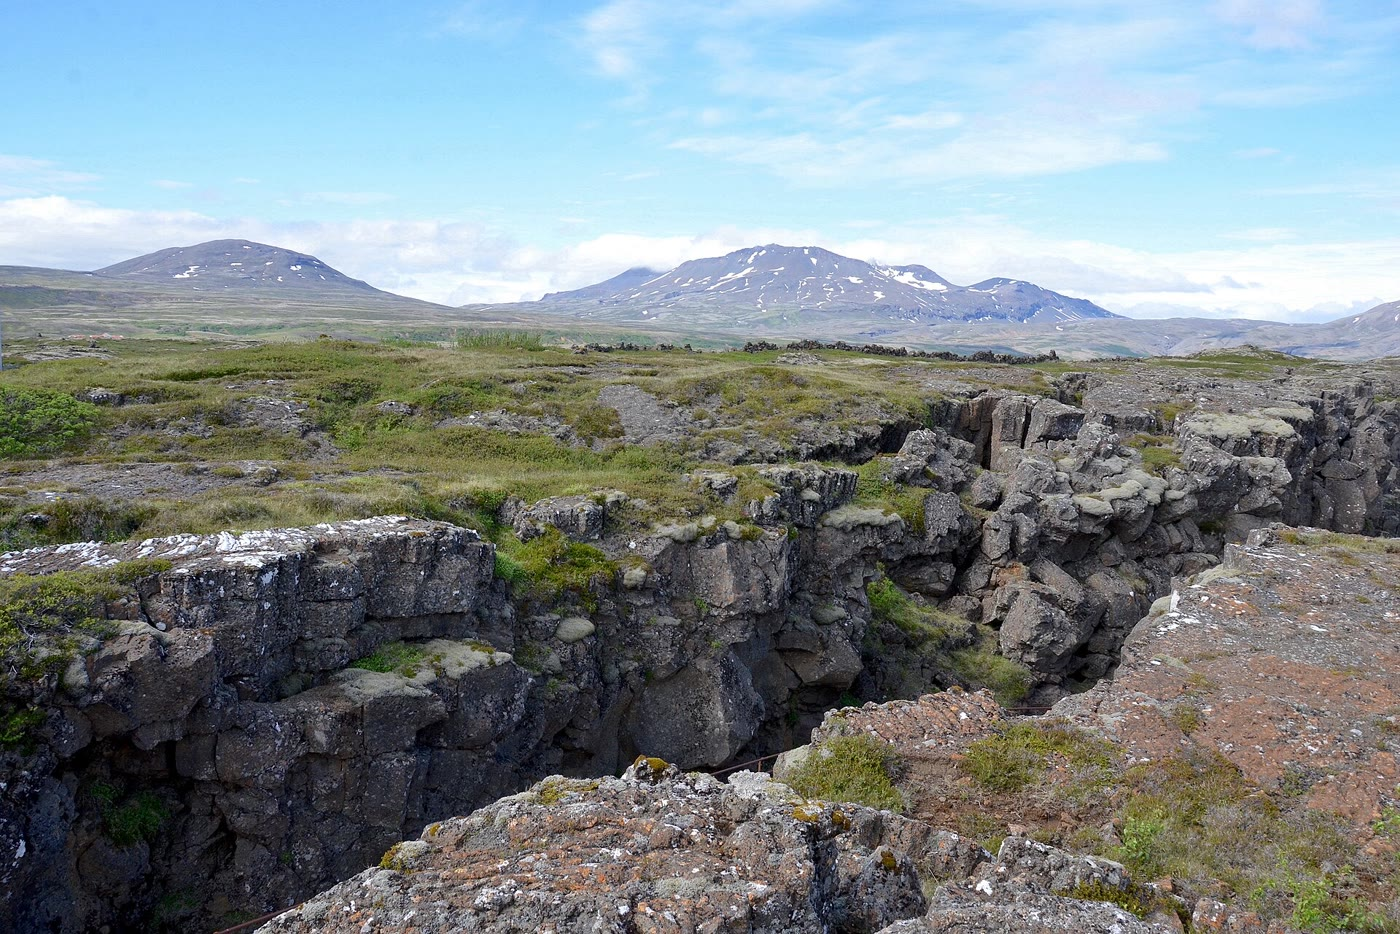
\includegraphics[width=0.8\linewidth]{images/book3/b1-thingvellir-fissure.jpg}

\par\smallskip{\small Rekahan terbuka di lantai lava lembah celah Þingvellir, di barat daya Islandia, tempat Punggungan Atlantik Tengah mencapai daratan. Aliran basal di lantai lembah dipotong oleh rekahan terbuka yang sejajar dengan celah. Foto: Olga Ernst, CC~BY-SA~4.0 (Wikimedia Commons).}
\label{fig:b1:rifts-ridges-margins:thingvellir}
\end{omfigure}
% ledger: commons:thingvellir

\subsection*{Celah gunung api dan celah miskin magma}

Celah berbeda dalam jumlah magma yang mereka terima. Pada celah \emph{miskin magma} peregangan ditanggung oleh sesar, dan \omterm{def:b1:layered-earth:layers}{kerak} menipis ketika blok-blok saling tergelincir. Pada celah gunung api, magma mengambil alih: dike menerobos \omterm{def:b1:layered-earth:layers}{kerak} sepanjang sumbu, masing-masing membuka celah sebesar ketebalannya sendiri, dan lava membanjiri permukaan. Celah Afrika Timur memperlihatkan keduanya berdampingan: cabang timurnya sangat vulkanik, sedangkan cabang baratnya kurang demikian dan memuat basin sedimen yang dalam, terisi oleh danau seperti Danau Tanganyika dan dibatasi oleh sesar.
% ledger: roberts:ear

Kedua cabang mulai terbentuk sekitar 25 juta tahun yang lalu, dan celah itu membelah lempeng Afrika menjadi lempeng Nubia di barat dan lempeng Somalia di timur. Dari sambungan tiga Afar, celah itu berjalan ke selatan, dalam dua cabang yang mengelilingi kraton Tanzania yang tua, tebal dan dingin. Geraknya lambat: dihitung dari vektor lempeng Somalia dan Nubia, masing-masing diukur relatif terhadap lempeng Antartika, Somalia menjauh dari Nubia sebesar \qty{6.0}{mm.yr^{-1}} ke arah \ang{105} di Etiopia tengah (\ang{8.5}\,LU, \ang{39.5}\,BT), dan sebesar \qty{5.1}{mm.yr^{-1}} di khatulistiwa. Banyak gempa bumi di celah ini menunjukkan sesar normal.
% ledger: roberts:ear, morvel:sm-an, morvel:nb-an (SM-NB from SM-AN minus NB-AN, computed with figdata/bachelor-1/euler_velocities.py)

Di Afar, di ujung utara, celah bertemu dengan Laut Merah dan Teluk Aden. Sebagian besar basal banjir Etiopia meletus di sana sekitar 30 juta tahun yang lalu, dalam satu juta tahun atau kurang, dan magma terus berdatangan sejak itu: aliran lava di permukaan, terobosan di dalam \omterm{def:b1:layered-earth:layers}{kerak}, dan material baru yang ditambahkan di bawahnya, sebanyak itu sehingga \omterm{def:b1:layered-earth:layers}{kerak} yang diterobos tetap mempertahankan ketebalannya selama tahap awal pemekaran. Krisis 2005 memperlihatkan bagaimana celah seperti itu terbuka: tidak secara mantap, melainkan dalam episode, masing-masing berupa dike selebar meter yang menerobos dalam hitungan hari atau minggu. Karena lempeng-lempeng memisah sekitar \qty{18}{mm.yr^{-1}} di sana, dike 2005 setebal \qty{8}{m} menampung peregangan selama sekitar 440 tahun.
% ledger: hofmann:traps, bastow:afar, wright:afar, morvel:ar-nb (rate computed with euler_velocities.py)

\section{Perpecahan dan tepi pasif}

Jika peregangan berlanjut, \omterm{def:b1:layered-earth:layers}{kerak} benua menipis hingga habis, \omterm{def:b1:layered-earth:layers}{mantel} naik di bawah celah dan meleleh ketika naik, dan \omterm{def:b1:rifts-ridges-margins:oceanic-crust}{kerak samudra} pertama terbentuk di antara kedua belahan benua. Saat itulah \emph{perpecahan} terjadi. Sejak itu lempeng-lempeng bergerak menjauh di sebuah punggungan di tengah samudra baru, dan kedua tepi benua, yang terbawa menjauh dari punggungan, berhenti menjadi batas lempeng.

\begin{definition}[Tepi pasif, transisi samudra--benua, ketidakselarasan perpecahan]\label{def:b1:rifts-ridges-margins:passive-margin}
Sebuah \emph{tepi pasif}\index{tepi pasif} adalah tepi benua yang terbentuk oleh pemekaran dan tidak lagi menjadi batas lempeng: benua dan dasar samudra di sebelahnya termasuk lempeng yang sama. \emph{Transisi samudra--benua}\index{transisi samudra--benua} adalah zona pada tepi itu, beberapa kilometer hingga puluhan kilometer lebarnya, antara \omterm{def:b1:layered-earth:layers}{kerak} benua yang menipis dan \omterm{def:b1:rifts-ridges-margins:oceanic-crust}{kerak samudra} normal. \emph{Ketidakselarasan perpecahan}\index{ketidakselarasan perpecahan} adalah \omterm{def:b1:cross-sections:unconformity}{ketidakselarasan} yang memisahkan sedimen yang diendapkan di basin celah, miring bersama blok-blok, dari sedimen yang tidak terganggu dan diletakkan di atas tepi setelah perpecahan.
\end{definition}

\omterm{def:b1:rifts-ridges-margins:passive-margin}{Tepi pasif} membentang di sebagian besar Atlantik, Samudra Arktik dan bagian barat Samudra Hindia, serta hampir seluruh pantai Afrika, Australia, Greenland dan India. Tepi timur Amerika Utara dan tepi barat laut Afrika adalah dua sisi dari satu celah: keduanya disebut tepi \emph{konjugat}. Profilnya adalah urutan yang sudah dikenal dari dasar samudra dekat daratan: paparan benua, lereng, tanjakan dan dataran abisal. Di bawah paparan dan lereng terdapat \omterm{def:b1:layered-earth:layers}{kerak} benua yang menipis, terpotong oleh sesar normal yang miring ke arah samudra, dengan blok-blok berputar yang terkubur di bawah sedimen.

\begin{omfigure}
\begin{tikzpicture}[x=0.95cm, y=0.9cm, font=\scriptsize]
% (a) continental rift: half-grabens on east-dipping faults; coordinates from calc/fig13_margin.py
\begin{scope}
\fill[green!25!gray!45] (0,-2) -- (3,-2) -- (6,-1.75) -- (9,-2) -- (12,-2) -- (12,-2.5) -- (0,-2.5) -- cycle;
\fill[orange!22] (0,0) -- (3.5,0) -- (3.931,-0.8) -- (4.75,-0.25) -- (5.05,-0.7) -- (6,-0.2) -- (6.223,-0.55) -- (7.25,-0.15) -- (7.402,-0.4) -- (8.6,0) -- (12,0) -- (12,-2) -- (9,-2) -- (6,-1.75) -- (3,-2) -- (0,-2) -- cycle;
\fill[yellow!45] (3.565,-0.12) -- (3.931,-0.8) -- (4.75,-0.25) -- (4.75,-0.12) -- cycle;
\fill[yellow!45] (4.75,-0.12) -- (4.75,-0.25) -- (5.05,-0.7) -- (6,-0.2) -- (6,-0.12) -- cycle;
\fill[yellow!45] (6,-0.12) -- (6,-0.2) -- (6.223,-0.55) -- (7.25,-0.15) -- (7.25,-0.12) -- cycle;
\fill[yellow!45] (7.25,-0.12) -- (7.25,-0.15) -- (7.402,-0.4) -- (8.241,-0.12) -- cycle;
\draw (0,0) -- (3.5,0) -- (3.931,-0.8) -- (4.75,-0.25) -- (5.05,-0.7) -- (6,-0.2) -- (6.223,-0.55) -- (7.25,-0.15) -- (7.402,-0.4) -- (8.6,0) -- (12,0);
\draw[contact] (0,-2) -- (3,-2) -- (6,-1.75) -- (9,-2) -- (12,-2);
\draw[fault] (3.5,0) -- (4.2,-1.3);
\draw[fault] (4.75,-0.25) -- (5.45,-1.3);
\draw[fault] (6,-0.2) -- (6.7,-1.3);
\draw[fault] (7.25,-0.15) -- (7.95,-1.3);
\node[anchor=west, font=\small\bfseries] at (0,0.75) {(a) celah benua};
\node[anchor=south] at (2.2,0) {bahu celah};
\node[anchor=south, align=center] at (6.3,0) {paruh-graben terisi sedimen};
\draw[-{Stealth[length=3pt]}] (2.6,-0.75) node[anchor=east] {sesar batas} -- (3.75,-0.5);
\node at (9.8,-1.0) {kerak benua};
\node at (10.3,-2.25) {mantel};
\node at (6,-2.18) {Moho terangkat di bawah celah};
\end{scope}
% (b) break-up: conjugate halves, the first oceanic crust between them
\begin{scope}[yshift=-3.6cm]
\fill[omSea!35] (2.8,0) -- (9.2,0) -- (9.2,-1.3) -- (2.8,-1.3) -- cycle;
\fill[green!25!gray!45] (0,-2) -- (2.5,-2) -- (5.5,-1.3) -- (6.5,-1.3) -- (9.5,-2) -- (12,-2) -- (12,-2.5) -- (0,-2.5) -- cycle;
\fill[orange!22] (0,0) -- (2.8,0) -- (3.146,-0.75) -- (3.8,-0.3) -- (4.13,-0.85) -- (4.7,-0.45) -- (5.053,-0.95) -- (5.5,-1) -- (5.5,-1.3) -- (2.5,-2) -- (0,-2) -- cycle;
\fill[orange!22] (12,0) -- (9.2,0) -- (8.854,-0.75) -- (8.2,-0.3) -- (7.87,-0.85) -- (7.3,-0.45) -- (6.947,-0.95) -- (6.5,-1) -- (6.5,-1.3) -- (9.5,-2) -- (12,-2) -- cycle;
\fill[lith basalt] (5.5,-1) -- (6.5,-1) -- (6.5,-1.3) -- (5.5,-1.3) -- cycle;
\draw (0,0) -- (2.8,0) -- (3.146,-0.75) -- (3.8,-0.3) -- (4.13,-0.85) -- (4.7,-0.45) -- (5.053,-0.95) -- (5.5,-1) -- (6.5,-1) -- (6.947,-0.95) -- (7.3,-0.45) -- (7.87,-0.85) -- (8.2,-0.3) -- (8.854,-0.75) -- (9.2,0) -- (12,0);
\draw[contact] (0,-2) -- (2.5,-2) -- (5.5,-1.3) -- (6.5,-1.3) -- (9.5,-2) -- (12,-2);
\draw[omSea!70!black] (2.8,0) -- (9.2,0);
\draw[fault] (2.8,0) -- (3.4,-1.3);
\draw[fault] (3.8,-0.3) -- (4.4,-1.3);
\draw[fault] (4.7,-0.45) -- (5.3,-1.3);
\draw[fault] (9.2,0) -- (8.6,-1.3);
\draw[fault] (8.2,-0.3) -- (7.6,-1.3);
\draw[fault] (7.3,-0.45) -- (6.7,-1.3);
\draw[omRidge, very thick, -{Stealth[length=3pt]}] (6,-2.3) -- (6,-1.45);
\node[anchor=west, font=\small\bfseries] at (0,0.75) {(b) perpecahan};
\node[anchor=south] at (6,0) {laut membanjiri celah};
\node[anchor=west] at (6.15,-2.1) {mantel naik dan meleleh};
\node[anchor=south, fill=white, fill opacity=0.8, text opacity=1, inner sep=1pt, align=center] at (6,-0.85) {kerak samudra\\pertama};
\node at (1.4,-1.0) {blok miring};
\node at (10.6,-1.0) {blok miring};
\node at (1.4,-2.25) {mantel};
\end{scope}
% (c) one passive margin after drift
\begin{scope}[yshift=-7.4cm]
\fill[omSea!35] (1.2,0.3) -- (12,0.3) -- (12,-1.2) -- (8.2,-1.15) -- (6.4,-0.9) -- (4.6,0.1) -- cycle;
\fill[green!25!gray!45] (0,-2.3) -- (2,-2.3) -- (5.9,-1.8) -- (6.7,-2.1) -- (12,-2.1) -- (12,-2.7) -- (0,-2.7) -- cycle;
\fill[orange!22] (0,0.3) -- (1.2,0.3) -- (2.2,0) -- (3,-0.25) -- (3.259,-0.95) -- (4,-0.55) -- (4.286,-1.15) -- (4.9,-0.85) -- (5.233,-1.35) -- (5.9,-1.55) -- (5.9,-1.8) -- (2,-2.3) -- (0,-2.3) -- cycle;
\fill[pattern=crosshatch dots, pattern color=green!40!black] (5.9,-1.55) -- (6.4,-1.75) -- (6.7,-2.1) -- (5.9,-1.8) -- cycle;
\fill[lith basalt] (6.4,-1.75) -- (12,-1.75) -- (12,-2.1) -- (6.7,-2.1) -- cycle;
\fill[yellow!45] (3,-0.25) -- (3.259,-0.95) -- (4,-0.55) -- cycle;
\fill[yellow!45] (4,-0.55) -- (4.286,-1.15) -- (4.9,-0.85) -- cycle;
\fill[yellow!45] (4.9,-0.85) -- (5.233,-1.35) -- (5.9,-1.55) -- (5.9,-1.45) -- cycle;
\fill[yellow!15] (1.2,0.3) -- (4.6,0.1) -- (6.4,-0.9) -- (8.2,-1.15) -- (12,-1.2) -- (12,-1.75) -- (6.4,-1.75) -- (5.9,-1.55) -- (5.9,-1.45) -- (4.9,-0.85) -- (4,-0.55) -- (3,-0.25) -- (2.2,0) -- cycle;
\draw[black!45] (2.4,0.12) -- (4.8,-0.1) -- (6.6,-1.05) -- (8.4,-1.27) -- (12,-1.31);
\draw (1.2,0.3) -- (4.6,0.1) -- (6.4,-0.9) -- (8.2,-1.15) -- (12,-1.2);
\draw[omSea!70!black] (1.2,0.3) -- (12,0.3);
\draw[unconformity] (2.2,0) -- (3,-0.25) -- (4,-0.55) -- (4.9,-0.85) -- (5.9,-1.45);
\draw (3.259,-0.95) -- (4,-0.55) (4.286,-1.15) -- (4.9,-0.85) (5.233,-1.35) -- (5.9,-1.55) -- (6.4,-1.75) -- (12,-1.75);
\draw[contact] (0,-2.3) -- (2,-2.3) -- (5.9,-1.8) -- (6.7,-2.1) -- (12,-2.1);
\draw[fault] (3,-0.25) -- (3.5,-1.6);
\draw[fault] (4,-0.55) -- (4.5,-1.6);
\draw[fault] (4.9,-0.85) -- (5.4,-1.6);
\node[anchor=west, font=\small\bfseries] at (0,0.95) {(c) tepi pasif};
\node[anchor=south] at (3.4,0.25) {paparan};
\node[anchor=south west] at (5.6,-0.45) {lereng};
\node[anchor=south] at (8.4,-1.12) {tanjakan};
\node[anchor=south] at (10.6,-1.17) {dataran abisal};
\node[anchor=south] at (10.6,-0.1) {samudra};
\node at (9.8,-1.53) {sedimen pascacelah};
\node[fill=white, fill opacity=0.8, text opacity=1, inner sep=1pt, align=center] (bu) at (1.0,-0.6) {ketidakselarasan\\perpecahan};
\draw[-{Stealth[length=3pt]}] (bu.east) -- (2.55,-0.16);
\node[fill=white, fill opacity=0.8, text opacity=1, inner sep=1pt, align=center] (sr) at (1.6,-1.35) {sedimen\\sin-celah};
\draw[-{Stealth[length=3pt]}] (sr.east) -- (3.45,-0.75);
\node at (1.3,-1.98) {kerak benua};
\draw[decorate, decoration={brace, amplitude=3pt, mirror}] (5.9,-2.17) -- (6.7,-2.17) node[midway, below=3pt, align=center] {transisi\\samudra--benua};
\node[anchor=west, fill=white, fill opacity=0.85, text opacity=1, inner sep=1pt] at (8.6,-1.93) {kerak samudra};
\node at (3.6,-2.5) {mantel};
\end{scope}
\end{tikzpicture}

\par\smallskip{\small Dari celah ke \omterm{def:b1:rifts-ridges-margins:passive-margin}{tepi pasif} (gambar, tidak sesuai skala; ketinggian dibesar-besarkan). (a) \omterm{def:b1:layered-earth:layers}{Kerak} atas yang rapuh pecah di sepanjang sesar normal; blok-blok miring menjadi \omterm{def:b1:rifts-ridges-margins:rift}{paruh-graben} yang terisi sedimen, dan \omterm{def:b1:layered-earth:discontinuity}{Moho} naik di bawah \omterm{def:b1:layered-earth:layers}{kerak} yang menipis. (b) Pada perpecahan, \omterm{def:b1:layered-earth:layers}{kerak} benua terputus; laut membanjiri celah dan \omterm{def:b1:rifts-ridges-margins:oceanic-crust}{kerak samudra} pertama terbentuk. (c) Salah satu dari dua tepi, yang terbawa menjauh dari punggungan: blok-blok miringnya dan sedimennya terletak di bawah \omterm{def:b1:rifts-ridges-margins:passive-margin}{ketidakselarasan perpecahan}, tertimbun oleh sedimen pascacelah paparan, lereng dan tanjakan.}
\label{fig:b1:rifts-ridges-margins:margin}
\end{omfigure}

\subsection*{Dua jenis tepi}

Tepi mewarisi karakter celahnya. Pada tepi \emph{miskin magma}, seperti tepi Iberia dan Newfoundland, penampang seismik memperlihatkan blok-blok berputar yang lapisannya miring ke arah benua; di beberapa tempat \omterm{def:b1:rifts-ridges-margins:passive-margin}{transisi samudra--benua} dialasi oleh peridotit \omterm{def:b1:layered-earth:layers}{mantel}, yang terangkat ke dasar laut dan diubah oleh air laut menjadi serpentinit. Pada tepi \emph{gunung api}, seperti tepi Norwegia tengah, Greenland Timur, Namibia dan Brasil, transisi itu dibangun oleh basal: tumpukan aliran lava yang miring ke arah samudra, reflektor yang miring ke laut pada penampang seismik, dan di bawahnya \omterm{def:b1:layered-earth:layers}{kerak} bawah tempat gelombang P merambat luar biasa cepat, magma yang ditambahkan di bawah \omterm{def:b1:layered-earth:layers}{kerak} saat perpecahan. Tepi gunung api sedikit turun saat perpecahan.

\begin{inthefield}[Mencari tepi benua]
\omterm{def:b1:rifts-ridges-margins:passive-margin}{Transisi samudra--benua} terletak di bawah beberapa kilometer air dan sedimen, dan hanya ditemukan dengan geofisika, biasanya dengan beberapa metode sekaligus. Refleksi seismik mencitrakan blok-blok miring, \omterm{def:b1:rifts-ridges-margins:passive-margin}{ketidakselarasan perpecahan} dan, bila sinyalnya mencapai cukup dalam, \omterm{def:b1:layered-earth:discontinuity}{Moho}. Refraksi seismik sudut lebar mengukur kecepatan gelombang P melalui \omterm{def:b1:layered-earth:layers}{kerak}, yang berbeda antara \omterm{def:b1:layered-earth:layers}{kerak} benua dan \omterm{def:b1:rifts-ridges-margins:oceanic-crust}{kerak samudra}. Data gravitasi, yang diinversi untuk kedalaman \omterm{def:b1:layered-earth:discontinuity}{Moho}, memberikan ketebalan \omterm{def:b1:layered-earth:layers}{kerak}. Garis-garis magnetik dasar samudra berhenti di tempat \omterm{def:b1:layered-earth:layers}{kerak} benua, yang tenang secara magnetik, mulai.
\end{inthefield}

Setelah perpecahan, sebuah tepi tenggelam. Selama pemekaran, \omterm{def:b1:layered-earth:lithosphere}{litosfer} menipis dan memanas; terbawa menjauh dari punggungan, ia mendingin dan menyusut, seperti dasar samudra di sebelahnya, dan ruang yang terbuka di atasnya terisi oleh baji sedimen pascacelah, yang beratnya menekannya lebih jauh ke bawah. Bagian pendinginan dari kisah ini dituturkan di \cref{sec:b1:rifts-ridges-margins:depth-age}; berat sedimen menjadi pokok bahasan \cref{ch:b1:diagenesis-basins}.

\section{Punggungan cepat dan lambat}

Setelah samudra lahir, ia tumbuh di punggungannya. Punggungan menyebar dengan laju yang sangat berbeda: laju yang diukur selama beberapa juta tahun terakhir berkisar dari \qty{9.7}{mm.yr^{-1}} di Laut Merah utara hingga \qty{154.4}{mm.yr^{-1}} di Punggungan Pasifik Timur. Bentuknya bergantung pada laju itu.
% ledger: morvel:range

\begin{definition}[Punggungan menyebar cepat, lambat dan sangat lambat]\label{def:b1:rifts-ridges-margins:ridge-classes}
Sebuah punggungan diklasifikasikan menurut \omterm{def:b1:plate-kinematics:spreading-rate}{laju penyebaran penuhnya}. Sebuah \emph{punggungan menyebar sangat lambat}\index{punggungan menyebar sangat lambat} membuka dengan kurang dari sekitar \qty{20}{mm.yr^{-1}}; sebuah \emph{punggungan menyebar lambat}\index{punggungan menyebar lambat} pada 20 hingga \qty{55}{mm.yr^{-1}}; punggungan menengah pada 55 hingga \qty{75}{mm.yr^{-1}}; sebuah \emph{punggungan menyebar cepat}\index{punggungan menyebar cepat} pada lebih dari sekitar \qty{75}{mm.yr^{-1}}.
\end{definition}
% ledger: seton:rate-classes, dick:ultraslow

Batasnya adalah konvensi dan berbeda antar penulis. Yang tidak berbeda adalah perubahan bentuknya. Punggungan lambat, seperti Punggungan Atlantik Tengah, memiliki lembah aksial di antara sesar normal yang menghadap ke dalam: celah di antara lempeng tidak segera terisi magma secepat ia terbuka, dan \omterm{def:b1:layered-earth:lithosphere}{litosfer} yang dingin pecah. Punggungan cepat, seperti Punggungan Pasifik Timur, tidak memiliki lembah celah tetapi tinggian aksial yang halus di atas lensa lelehan, diisi ulang cukup sering untuk mengimbangi. Bagaimanapun juga sumbunya terletak sekitar \qty{2500}{m} di bawah permukaan laut, dan dasar tertua cekungan samudra hampir \qty{4}{km} lebih dalam (\cref{sec:b1:rifts-ridges-margins:depth-age}).
% ledger: parsons:plate-model (6400 - 2500 m)

Punggungan sangat lambat memperlihatkan apa yang terjadi ketika magma paling sedikit: vulkanismenya terputus-putus, mereka tidak memiliki \omterm{def:b1:rifts-ridges-margins:transform}{sesar transform}, dan di wilayah yang luas \omterm{def:b1:layered-earth:layers}{mantel} itu sendiri terangkat ke dasar laut. Punggungan Gakkel, di bawah Samudra Arktik, yang paling lambat dari semuanya, sama sekali tidak terpotong; di sepanjang bagian tengah sumbunya yang panjangnya sekitar \qty{300}{km}, peridotit \omterm{def:b1:layered-earth:layers}{mantel} terletak langsung di sumbu, di antara vulkanisme yang melimpah di barat dan gunung api besar yang tersebar jarang di timur. Terutama di punggungan lambat dan sangat lambat, sebagian penyebaran ditanggung oleh sesar normal panjang yang landai, sesar pelepasan, yang dinding bawahnya tertarik keluar dari bawah sumbu: gabro dan peridotit mencapai dasar laut dalam kubah bergelombang, \emph{kompleks inti samudra}. Massif Atlantis, di samping Punggungan Atlantik Tengah dekat \ang{30}\,LU, adalah salah satunya: di puncaknya, pada \omterm{def:b1:layered-earth:layers}{kerak} berumur \qty{1.5}{Ma} sekitar \qty{15}{km} dari sumbu, air laut yang bereaksi dengan batuan \omterm{def:b1:layered-earth:layers}{mantel} memasok mata air hangat dan basa dari medan hidrotermal Lost City.
% ledger: dick:ultraslow, michael:gakkel, kelley:lost-city

\subsection*{Kerak samudra}

\begin{definition}[Kerak samudra, lava bantal, kompleks dike berlapis]\label{def:b1:rifts-ridges-margins:oceanic-crust}
\emph{Kerak samudra}\index{kerak samudra} adalah \omterm{def:b1:layered-earth:layers}{kerak} yang dibuat di punggungan samudra: 6 hingga \qty{7}{km} basal dan gabro, dari dasar laut hingga \omterm{def:b1:layered-earth:discontinuity}{Moho}, di bawah selimut sedimen. \emph{Lava bantal}\index{lava bantal} adalah lava yang meletus di bawah air, terdiri dari tabung dan lobus bulat yang saling terhubung, masing-masing dengan kulit kaca yang didinginkan oleh laut. \emph{Kompleks dike berlapis}\index{kompleks dike berlapis} adalah lapisan yang hampir seluruhnya terdiri dari dike vertikal sejajar, masing-masing menerobos dike sebelumnya.
\end{definition}

Lapisan \omterm{def:b1:rifts-ridges-margins:oceanic-crust}{kerak samudra} pertama kali didefinisikan oleh seismologi, lalu diambil sampelnya dengan pengeboran dan dikenali pada irisan dasar samudra yang terdorong ke atas benua, yaitu ofiolit. Dari atas:
\begin{itemize}
  \item lapisan~1, sedimen, tipis atau tidak ada dekat punggungan dan menebal seiring umur dasar;
  \item lapisan~2, rata-rata \qty{1.84}{km} basal: \omterm{def:b1:rifts-ridges-margins:oceanic-crust}{lava bantal} di bagian atas
        (lapisan~2A), dike diabas di bawahnya (lapisan~2B);
  \item lapisan~3, empat hingga lima kilometer sisanya, berupa gabro dan, di dasarnya,
        kumulat yang mengendap dari magma: sekitar \qty{70}{\percent} dari ketebalan
        \omterm{def:b1:layered-earth:layers}{kerak}.
\end{itemize}
Di bawah \omterm{def:b1:layered-earth:discontinuity}{Moho} terdapat peridotit \omterm{def:b1:layered-earth:layers}{mantel}, residu yang tertinggal oleh peleburan.
% ledger: christeson:crust, white:crust (layer 3: 6.15 - 1.84 = 4.3 km, 70 %; 7.1 - 1.84 = 5.3 km)

Refraksi seismik memberikan ketebalan rata-rata \omterm{def:b1:layered-earth:layers}{kerak} beku sebesar \qty[uncertainty-mode=separate]{7.1 \pm 0.8}{km} jauh dari \omterm{def:b1:rifts-ridges-margins:transform}{zona patahan} dan titik panas, dan suatu sintesis profil seismik yang lebih baru sebesar \qty{6.15}{km}, hampir sama di semua laju penyebaran: jumlah lelehan bergantung pada suhu \omterm{def:b1:layered-earth:layers}{mantel} yang naik, bukan pada kecepatan naiknya. Hanya punggungan yang sangat lambat membuat \omterm{def:b1:layered-earth:layers}{kerak} yang anomali tipisnya: \omterm{def:b1:layered-earth:layers}{mantel} di sana punya waktu untuk mendingin saat naik, dan meleleh lebih sedikit. Di atas plume panas, \omterm{def:b1:layered-earth:layers}{kerak} lebih tebal, sekitar \qty{20}{km} tepat di atas inti plume yang naik, seperti di bawah Islandia (\cref{ch:b1:hotspots}). Di seluruh punggungan secara bersama-sama, sekitar \qty{3.0}{km^2} dasar laut baru dan sekitar \qty{20}{km^3} \omterm{def:b1:layered-earth:layers}{kerak} baru dibuat setiap tahun.
% ledger: white:crust, christeson:crust, data:pb2002 (production summed over the spreading steps in figdata/bachelor-1/ridge_budget.py)

\begin{omfigure}
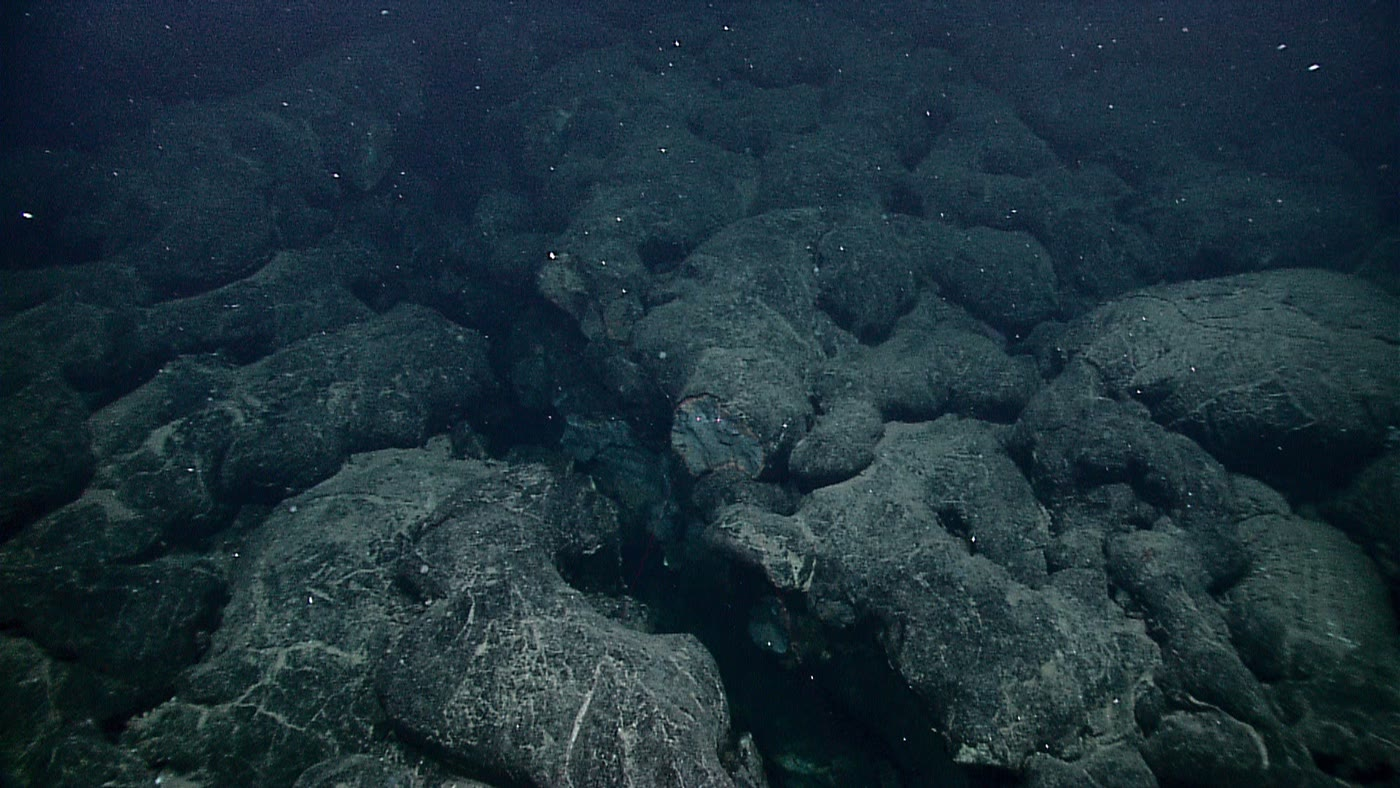
\includegraphics[width=0.6\linewidth]{images/book3/b1-pillow-lava.jpg}

\par\smallskip{\small \omterm{def:b1:rifts-ridges-margins:oceanic-crust}{Lava bantal} di Celah Galápagos, terpotong oleh rekahan yang terbuka setelah lava itu mengeras: puncak lapisan~2 \omterm{def:b1:rifts-ridges-margins:oceanic-crust}{kerak samudra} saat terbentuk. Setiap bantal adalah lidah lava yang dibekukan dari luar oleh air laut. Foto: NOAA Okeanos Explorer Program, Galápagos Rift Expedition 2011, CC~BY~2.0 (Wikimedia Commons).}
\label{fig:b1:rifts-ridges-margins:pillows}
\end{omfigure}
% ledger: commons:pillow-expl6453

\begin{proposition}[Setiap dike membelah yang sebelumnya]\label{prop:b1:rifts-ridges-margins:dykes}
Anggaplah setiap dike dari \omterm{def:b1:rifts-ridges-margins:oceanic-crust}{kompleks dike berlapis} disuntikkan di sepanjang sumbu penyebaran, tempat \omterm{def:b1:layered-earth:layers}{kerak} paling panas dan paling lemah, dan \omterm{def:b1:layered-earth:layers}{kerak} bergerak menjauhi sumbu secara simetris. Maka sebagian besar dike ditemukan terbelah dua, masing-masing setengahnya hanya memiliki tepi yang didinginkan di sisi tetangganya yang lebih tua.
\end{proposition}

\begin{proof}
Sebuah dike mendingin terhadap batuan yang lebih dingin di kedua sisinya: ia memiliki dua tepi dingin ketika terbentuk. Dike berikutnya naik di tempat \omterm{def:b1:layered-earth:layers}{kerak} paling lemah, di sepanjang sumbu, yaitu melalui tengah dike sebelumnya, batuan yang masih paling panas. Ia membelahnya menjadi dua setengah, yang dibawa menjauh oleh penyebaran ke masing-masing sisi; setiap setengah tetap memiliki tepi dingin di sisi luarnya dan, di sisi dalamnya, \omterm{def:b1:geological-maps:geological-map}{kontak} yang belum mendingin dengan dike baru. Setiap dike kecuali yang terakhir terbelah dengan cara ini.
\end{proof}

Dike dengan tepi dingin hanya di satu sisi memang merupakan aturan dalam \omterm{def:b1:rifts-ridges-margins:oceanic-crust}{kompleks dike berlapis}: tanda \omterm{def:b1:layered-earth:layers}{kerak} yang dibangun, dike demi dike, oleh penyebaran.


\section{Hukum kedalaman--umur}\label{sec:b1:rifts-ridges-margins:depth-age}

Dasar samudra dangkal di punggungan dan dalam jauh darinya. Karena dasar dibuat di punggungan lalu dibawa menjauh, jarak dari punggungan adalah umur, dan kedalaman dasar bergantung pada umurnya. Lempeng mendingin dari atas seiring bertambahnya umur (\cref{ch:b1:heat-budget}); batuan dingin lebih padat, dan kolom yang lebih padat mengapung lebih rendah.

\begin{lemma}[Sebuah integral fungsi galat]\label{lem:b1:rifts-ridges-margins:erfc}
With $\operatorname{erfc} u = 1 - \operatorname{erf} u =
\frac{2}{\sqrt\pi}\int_u^\infty e^{-s^2}\,\mathrm ds$,
\[
  \int_0^\infty \operatorname{erfc} u \,\mathrm du = \frac{1}{\sqrt\pi}.
\]
\end{lemma}

\begin{proof}
Turunan dari $\operatorname{erfc}$ adalah $-\frac{2}{\sqrt\pi}e^{-u^2}$.
Dengan integrasi parsial pada $[0, X]$,
\[
  \int_0^X \operatorname{erfc} u\,\mathrm du
  = \bigl[u \operatorname{erfc} u\bigr]_0^X + \frac{2}{\sqrt\pi}\int_0^X u\,e^{-u^2}\,\mathrm du
  = X\operatorname{erfc} X + \frac{1}{\sqrt\pi}\bigl(1 - e^{-X^2}\bigr).
\]
Untuk $X > 0$ dan $s \ge X$, $e^{-s^2} \le (s/X)e^{-s^2}$, sehingga
$X\operatorname{erfc} X \le \frac{2}{\sqrt\pi}\int_X^\infty s\,e^{-s^2}\,\mathrm ds
= e^{-X^2}/\sqrt\pi$, yang menuju 0. Membiarkan $X \to \infty$ menghasilkan hasilnya.
\end{proof}

\begin{theorem}[Hukum kedalaman--umur]\label{thm:b1:rifts-ridges-margins:depth-age}
Anggaplah bahwa
\begin{enumerate}
  \item \omterm{def:b1:layered-earth:layers}{mantel} meninggalkan punggungan pada suhu seragam $T_m$, dan lempeng samudra
        berumur $t$ adalah setengah-ruang yang sejak itu didinginkan dari
        permukaannya, dipertahankan pada $T_0$, dengan difusivitas termal $\kappa$;
  \item massa jenis batuan yang didinginkan adalah $\rho_m\bigl(1 + \alpha(T_m -
        T)\bigr)$, dengan $\rho_m$ massa jenis \omterm{def:b1:layered-earth:layers}{mantel} pada $T_m$ dan
        $\alpha$ koefisien muai termalnya;
  \item setiap kolom berada dalam kesetimbangan isostatik di atas \omterm{def:b1:isostasy-gravity:isostasy}{kedalaman
        kompensasi} yang terletak di bawah lapisan yang mendingin, dan air laut
        memiliki massa jenis $\rho_w$.
\end{enumerate}
Maka kedalaman dasar laut berumur $t$ adalah
\[
  d(t) = d_r + C\sqrt t, \qquad
  C = \frac{2}{\sqrt\pi}\,\frac{\rho_m\,\alpha\,(T_m - T_0)\sqrt\kappa}{\rho_m - \rho_w},
\]
di mana $d_r$ adalah kedalaman sumbu punggungan. Ini adalah
\emph{hukum kedalaman--umur}\index{hukum kedalaman--umur} dasar samudra.
\end{theorem}

\begin{proof}
Suhu dalam setengah-ruang yang mendingin adalah
\[
  T(z, t) = T_0 + (T_m - T_0)\operatorname{erf}\frac{z}{2\sqrt{\kappa t}},
\]
dengan $z$ kedalaman di bawah dasar laut; solusi persamaan panas ini diterima di sini, seperti di \cref{ch:b1:heat-budget}, dan diturunkan dalam volume Tahun ke-3. Bandingkan kolom di punggungan, terdiri dari air hingga $d_r$ dan \omterm{def:b1:layered-earth:layers}{mantel} bersuhu $T_m$ di bawahnya, dengan kolom berumur $t$, terdiri dari air hingga $d$ dan lempeng yang mendingin di bawahnya, keduanya hingga \omterm{def:b1:isostasy-gravity:isostasy}{kedalaman kompensasi} $D$. Massa per satuan luas keduanya sama:
\[
  \rho_w d_r + \rho_m (D - d_r) = \rho_w d + \int_0^{D-d}\rho_m\bigl(1 + \alpha(T_m - T)\bigr)\mathrm dz
  = \rho_w d + \rho_m (D - d) + \rho_m\alpha\int_0^{D-d}(T_m - T)\,\mathrm dz.
\]
Maka
\[
  (\rho_m - \rho_w)(d - d_r) = \rho_m\alpha\int_0^{D-d}(T_m - T)\,\mathrm dz.
\]
Karena $T_m - T = (T_m - T_0)\operatorname{erfc}\bigl(z/2\sqrt{\kappa t}\bigr)$ dapat diabaikan di bawah lapisan yang mendingin, integral itu boleh dibawa sampai tak hingga; dengan $u = z/2\sqrt{\kappa t}$ dan \cref{lem:b1:rifts-ridges-margins:erfc},
\[
  \int_0^\infty (T_m - T)\,\mathrm dz = (T_m - T_0)\,2\sqrt{\kappa t}\int_0^\infty\operatorname{erfc}u\,\mathrm du
  = \frac{2}{\sqrt\pi}(T_m - T_0)\sqrt{\kappa t}.
\]
Membagi dengan $\rho_m - \rho_w$ memberikan $d - d_r = C\sqrt t$.
\end{proof}

Air penting: ketika lempeng tenggelam, air mengisi ruang di atasnya, dan beratnya menekan lempeng lebih jauh ke bawah. Koefisien muai efektif $\alpha\rho_m/(\rho_m - \rho_w)$ lebih besar daripada $\alpha$ dengan faktor $3300/2300 \approx 1.43$.

Dengan $\alpha = \qty{3.2e-5}{K^{-1}}$, $T_m - T_0 = \qty{1350}{K}$,
$\kappa = \qty{e-6}{m^2.s^{-1}}$, $\rho_m = \qty{3300}{kg.m^{-3}}$ dan
$\rho_w = \qty{1000}{kg.m^{-3}}$, serta waktu dihitung dalam juta tahun
($\sqrt{\kappa\times\qty{1}{Ma}} = \qty{5618}{m}$), teorema memberikan
$C = \qty{393}{m.Ma^{-1/2}}$. Konstanta yang dicocokkan oleh Parsons dan Sclater
dengan kedalaman Pasifik Utara dan Atlantik Utara, setelah sedimennya dibuang,
cukup dekat: $d_r \approx \qty{2500}{m}$ dan
$C \approx \qty{350}{m.Ma^{-1/2}}$, dari 0 hingga \qty{70}{Ma}. Nilai
$\alpha$ dan $T_m$ yang dipakai di atas adalah nilai model lempeng mereka untuk
dasar tua, \omterm{def:b1:layered-earth:layers}{mantel} pada \qty{1350}{\degreeCelsius} dan
$\alpha = \qty{3.2e-5}{\per\degreeCelsius}$, yang tidak pasti masing-masing
sebesar seperlima dan sepertiga, sehingga kesesuaian 393 dengan 350 sebaik yang
dapat diharapkan.
% ledger: parsons:plate-model, ps77:depth-age

\begin{example}[Dasar samudra berumur 25 dan 100 juta tahun]\label{ex:b1:rifts-ridges-margins:depths}
Dengan $d = 2500 + 350\sqrt t$ (meter, $t$ dalam juta tahun), dasar berumur
\qty{25}{Ma} terletak pada $2500 + 350\times5 = \qty{4250}{m}$ dan dasar berumur
\qty{100}{Ma} pada $2500 + 350\times10 = \qty{6000}{m}$. Dasar tenggelam
\qty{1750}{m} dalam 25 juta tahun pertamanya, dan hanya \qty{1750}{m} lagi dalam
75 juta tahun berikutnya.
\end{example}
% ledger: parsons:plate-model

\begin{omfigure}
\begin{tikzpicture}
\begin{axis}[omrecord, omdepth, width=0.84\linewidth, height=6.6cm,
  xmin=0, xmax=13.6, ymin=2000, ymax=6800,
  xlabel={akar kuadrat umur dasar, $\sqrt t$ (\unit{Ma^{1/2}})},
  ylabel={kedalaman (\unit{m})},
  yticklabel style={/pgf/number format/set thousands separator={}},
  legend style={font=\scriptsize, at={(0.02,0.03)}, anchor=south west, draw=none, fill=white, fill opacity=0.85, text opacity=1},
  legend cell align=left]
% computed in figdata/bachelor-1/depth_age.py; ledger: data:etopo1, data:b2-seafloor-age, parsons:plate-model
\addplot[name path=lo, draw=none, forget plot] table[x expr=sqrt(\thisrow{t}), y=q1] {figdata/out/bachelor-1-depth_age-bins.dat};
\addplot[name path=hi, draw=none, forget plot] table[x expr=sqrt(\thisrow{t}), y=q3] {figdata/out/bachelor-1-depth_age-bins.dat};
\addplot[black!12] fill between[of=lo and hi];
\addlegendentry{setengah tengah sel}
\addplot[only marks, mark=*, mark size=1.1pt, black!70] table[x expr=sqrt(\thisrow{t}), y=median] {figdata/out/bachelor-1-depth_age-bins.dat};
\addlegendentry{median kedalaman, kelas umur 2-Ma}
\addplot[very thick, omProp] table[x expr=sqrt(\thisrow{t}), y=halfspace] {figdata/out/bachelor-1-depth_age-models.dat};
\addlegendentry{setengah-ruang, $2500 + 350\sqrt t$}
\addplot[thick, omDef, densely dashed] table[x expr=sqrt(\thisrow{t}), y=plate] {figdata/out/bachelor-1-depth_age-models.dat};
\addlegendentry{model lempeng, $6400 - 3200\,e^{-t/62.8}$}
\draw[black!50, densely dotted] (axis cs:8.944,2000) -- (axis cs:8.944,6800);
\node[font=\scriptsize, anchor=north west, black!70] at (axis cs:8.944,2060) {\qty{80}{Ma}};
\node[font=\scriptsize, anchor=north west, black!70] at (axis cs:4.472,2060) {\qty{20}{Ma}};
\draw[black!50, densely dotted] (axis cs:4.472,2000) -- (axis cs:4.472,6800);
\end{axis}
\end{tikzpicture}

\par\smallskip{\small Kedalaman dasar samudra terhadap akar kuadrat umurnya. Setiap titik adalah median kedalaman sel satu derajat dari samudra dunia yang dasarnya jatuh dalam kelas umur dua juta tahun (31\,538 sel, lebih dalam dari \qty{1000}{m}); pita abu-abu memuat setengah tengahnya. Hukum setengah-ruang berupa garis lurus dalam plot ini. Dasar muda mengikutinya dengan dekat; dasar yang lebih tua terletak di atasnya, karena sel-sel itu membawa sedimennya dan mencakup gunung laut serta dataran vulkanik, dan karena dasar tua berhenti tenggelam (putus-putus: model lempeng). Data: ETOPO1 (NOAA) dan umur dasar samudra dari Seton dan lainnya (2020).}
\label{fig:b1:rifts-ridges-margins:depth-age}
\end{omfigure}

Gambar ini menguji teorema pada seluruh samudra. Hingga sekitar \qty{20}{Ma} ($\sqrt t \approx 4.5$) median berada dalam sekitar seratus meter dari hukum. Garis lurus yang dicocokkan pada median yang lebih muda dari \qty{70}{Ma} memiliki \omterm{def:b1:geological-maps:attitude}{kemiringan} hanya \qty{250}{m.Ma^{-1/2}}: kedalaman yang terukur adalah kedalaman permukaan sedimen, sedangkan hukum memberikan kedalaman
puncak \omterm{def:b1:layered-earth:layers}{kerak}, dan selimut sedimen menebal seiring umur. Antara 60 dan \qty{80}{Ma}, dasar menyimpang dari hukum akar kuadrat meskipun sedimennya telah dibuang: ia menjadi lebih dangkal daripada hukum, dan berhenti tenggelam.
Model lempeng, yaitu lempeng setebal \qty{125}{km} yang dasarnya ditahan pada suhu \omterm{def:b1:layered-earth:layers}{mantel}, menggambarkan perataan ini: kedalamannya menuju sekitar \qty{6400}{m}, dan \omterm{def:b1:heat-budget:heat-flow}{aliran panasnya} menuju konstan, seolah panas dipasok ke dasar lempeng tua oleh \omterm{def:b1:layered-earth:layers}{mantel} yang berkonveksi. Model itu dipelajari dalam volume Tahun ke-3; dalam buku ini hukum akar kuadrat dipakai hingga \qty{80}{Ma}.
% ledger: parsons:plate-model; fit and cell count from depth_age.py (values part)

\begin{method}[Menentukan umur dasar samudra dari kedalamannya]\label{met:b1:rifts-ridges-margins:age-from-depth}
Untuk memperkirakan umur dasar samudra tempat anomali magnetiknya tidak ada atau belum dipetakan:
\begin{enumerate}
  \item ukur kedalaman dasar dan, dari profil seismik, ketebalan sedimennya; ambil
        kedalaman $d$ puncak \omterm{def:b1:layered-earth:layers}{kerak}, yang dikoreksi untuk berat sedimen;
  \item balik hukumnya: $t = \bigl((d - d_r)/C\bigr)^2$, dengan $d_r$ dan $C$ untuk
        samudra yang bersangkutan;
  \item periksa bahwa dasar lebih muda dari sekitar \qty{80}{Ma}, dan perkirakan
        ketidakpastiannya: galat $\delta d$ pada kedalaman memberikan
        $\delta t = 2t\,\delta d/(d - d_r)$.
\end{enumerate}
\end{method}

Untuk dasar pada \qty{4600}{m}, $t = (2100/350)^2 = \qty{36}{Ma}$, dan ketidakpastian \qty{100}{m} pada kedalaman memberikan $2\times36\times100/2100 \approx
\qty{3.4}{Ma}$ pada umur. Di tempat dasar lebih dangkal daripada yang diprediksi hukum pada wilayah yang luas, yaitu suatu tonjolan, penyebabnya bukan umur melainkan panas dari bawah (\cref{ch:b1:hotspots}).

Hukum ini juga menghubungkan samudra dengan permukaan laut. Punggungan yang menyebar lebih cepat membawa dasar muda dan dangkal lebih jauh dari sumbunya; cekungan samudra menampung lebih sedikit air, dan permukaan laut naik di atas benua. Selama puluhan juta tahun, perubahan laju penyebaran adalah salah satu dari dua penyebab utama perubahan permukaan laut global, bersama volume es di darat.

\section{Sesar transform dan zona patahan}

Punggungan bukanlah garis yang kontinu: ia terpotong menjadi segmen-segmen yang bergeser oleh sesar yang berjalan tegak lurus terhadapnya, searah penyebaran. Di luar pergeseran itu, sesar berlanjut sebagai bekas luka panjang melintasi dasar samudra.

\begin{definition}[Sesar transform, zona patahan]\label{def:b1:rifts-ridges-margins:transform}
Sebuah \emph{sesar transform}\index{sesar transform} adalah sesar geser-mendatar yang merupakan batas lempeng dan berakhir pada batas lempeng lain; transform punggungan--punggungan menghubungkan ujung dua segmen punggungan yang bergeser. Sebuah \emph{zona patahan}\index{zona patahan} adalah kelanjutan sesar transform di luar ujung segmen punggungan: lembah linear atau undakan melintasi dasar samudra yang memisahkan dasar berumur berbeda yang termasuk satu lempeng.
\end{definition}

\begin{proposition}[Pergeseran pada transform punggungan--punggungan]\label{prop:b1:rifts-ridges-margins:transform}
Dua segmen punggungan yang menyebar secara simetris pada setengah laju $u$, tegak lurus terhadap dirinya sendiri, bergeser oleh \omterm{def:b1:rifts-ridges-margins:transform}{sesar transform} sepanjang $a$. Maka:
\begin{enumerate}
  \item kedua sisi transform saling tergelincir pada laju penuh $2u$, dalam arah yang berlawanan dengan arah yang akan disarankan oleh pergeseran jika satu punggungan lurus telah terpotong dan digeser oleh sesar itu;
  \item sepanjang \omterm{def:b1:rifts-ridges-margins:transform}{zona patahan} kedua sisi tidak bergerak relatif satu sama lain, dan
        dasar di kedua sisi berbeda umur sebesar $a/u$;
  \item panjang transform tidak berubah seiring waktu.
\end{enumerate}
\end{proposition}

\begin{proof}
Ambil sumbu $x$ sepanjang transform, ke timur, dan sumbu $y$ ke utara, dalam kerangka punggungan. Biarkan segmen utara terletak pada $x = 0$, $y > 0$, dan segmen selatan pada $x = a$, $y < 0$ (pergeseran ke timur saat menuju selatan); transform adalah ruas $0 < x < a$ dari $y = 0$. Lempeng barat $W$ terletak di barat kedua segmen dan bergerak dengan $-u$ sepanjang $x$; lempeng timur $E$ terletak di timur keduanya dan bergerak dengan $+u$.

(1) Tepat di utara transform, pada $0 < x < a$, dasar terletak di timur segmen utara: ia termasuk $E$ dan bergerak ke timur dengan $u$. Tepat di selatannya, dasar terletak di barat segmen selatan: ia termasuk $W$ dan bergerak ke barat dengan $u$. Sisi utara bergerak ke timur dengan $2u$ relatif terhadap sisi selatan: dilihat dari kedua sisi, sisi yang jauh bergerak ke kanan, dan geraknya adalah geser-kanan (dekstral). Punggungan lurus yang terpotong oleh sesar, dengan bagian selatannya kini berada di timur bagian utaranya, justru akan mencatat pergeseran geser-kiri (sinistral).

(2) Untuk $x > a$, kedua sisi terletak di timur segmen mereka dan termasuk $E$: keduanya bergerak bersama. Pada jarak $x$ dari segmen utara, dasar di utara \omterm{def:b1:rifts-ridges-margins:transform}{zona patahan} berumur $x/u$; dasar di selatannya berada pada $x - a$ dari segmen selatan dan berumur $(x - a)/u$. Selisihnya adalah $a/u$. Hal yang sama berlaku untuk $x < 0$, tempat kedua sisi termasuk $W$.

(3) Kedua segmen tetap berada di $x = 0$ dan $x = a$ dalam kerangka punggungan, karena masing-masing menyebar secara simetris: transform mempertahankan panjang $a$.
\end{proof}

J.\ Tuzo Wilson melihat pada 1965 bahwa pergeseran punggungan tidak dapat dibaca sebagai pergeseran punggungan lurus yang lebih tua, dan ia memprediksi arah geser dalam proposisi itu; mekanisme fokal gempa bumi pada transform mengonfirmasinya. Gempa bumi terjadi di sepanjang transform yang aktif, di antara ujung-ujung punggungan; \omterm{def:b1:rifts-ridges-margins:transform}{zona patahan} biasanya tenang. Di seluruh \omterm{def:b1:rifts-ridges-margins:transform}{zona patahan}, dasar kedua sisinya berumur berbeda, dan karena itu, menurut \omterm{thm:b1:rifts-ridges-margins:depth-age}{hukum kedalaman--umur}, kedalamannya berbeda: undakan yang memudar perlahan dengan jarak dari punggungan. Di Atlantik Utara dekat \ang{52}\,LU, dua transform Charlie--Gibbs menggeser Punggungan Atlantik Tengah sekitar \qty{350}{km} secara keseluruhan.
% ledger: wilson:transform, data:pb2002 (offset summed over the transform steps in figdata/bachelor-1/ridge_budget.py)

\begin{omfigure}
\begin{tikzpicture}[x=0.95cm, y=0.95cm, font=\scriptsize]
\fill[omSea!10] (-5,-2.6) rectangle (8,2.6);
% isochrons (10 and 20 Ma), offset across the fracture zones
\foreach \x in {-4,-2,2,4} \draw[black!40] (\x,0) -- (\x,2.5);
\foreach \x in {-1,1,5,7} \draw[black!40] (\x,0) -- (\x,-2.5);
\node[black!55, anchor=south, fill=omSea!10, inner sep=1pt] at (2,2.0) {10};
\node[black!55, anchor=south, fill=omSea!10, inner sep=1pt] at (4,2.0) {20};
\node[black!55, anchor=south, fill=omSea!10, inner sep=1pt] at (-2,2.0) {10};
\node[black!55, anchor=south, fill=omSea!10, inner sep=1pt] at (-4,2.0) {20};
\node[black!55, anchor=north, fill=omSea!10, inner sep=1pt] at (5,-2.0) {10};
\node[black!55, anchor=north, fill=omSea!10, inner sep=1pt] at (7,-2.0) {20};
\node[black!55, anchor=north, fill=omSea!10, inner sep=1pt] at (1,-2.0) {10};
\node[black!55, anchor=north, fill=omSea!10, inner sep=1pt] at (-1,-2.0) {20};
% fracture zones and transform
\draw[black!60, thick, densely dashed] (-5,0) -- (0,0);
\draw[black!60, thick, densely dashed] (3,0) -- (8,0);
\draw[transform, line width=1.4pt] (0,0) -- (3,0);
% ridge segments
\draw[ridge, line width=1.1pt] (0,0) -- (0,2.6);
\draw[ridge, line width=1.1pt] (3,0) -- (3,-2.6);
\pic at (1.5,0) {dextral={90}};
\foreach \x in {0.4,0.75,2.25,2.6} \node[star, star points=5, star point ratio=2.2, fill=orange!90!black, draw=black, line width=0.2pt, inner sep=1.5pt] at (\x,0.0) {};
% plate motions
\draw[-{Stealth[length=4pt]}, very thick, black!70] (-2.8,1.1) -- (-3.9,1.1);
\draw[-{Stealth[length=4pt]}, very thick, black!70] (-0.2,-1.1) -- (-1.3,-1.1);
\draw[-{Stealth[length=4pt]}, very thick, black!70] (5.5,1.1) -- (6.6,1.1);
\draw[-{Stealth[length=4pt]}, very thick, black!70] (5.3,-1.1) -- (6.4,-1.1);
\node[font=\small] at (-3.3,1.55) {lempeng $W$};
\node[font=\small] at (6.1,1.55) {lempeng $E$};
\node[anchor=west, omRidge] at (0.1,2.25) {punggungan};
\node[anchor=east, omRidge] at (2.9,-2.25) {punggungan};
\node[anchor=north, align=center, fill=white, fill opacity=0.8, text opacity=1, inner sep=1pt] at (1.5,-0.35) {sesar transform\\(aktif, gempa bumi)};
\node[anchor=south, fill=white, fill opacity=0.8, text opacity=1, inner sep=1pt] at (5.5,0.12) {zona patahan (tidak aktif)};
\node[anchor=north, fill=white, fill opacity=0.8, text opacity=1, inner sep=1pt] at (-2.5,-0.12) {zona patahan (tidak aktif)};
\node[anchor=south, black!70, fill=omSea!10, inner sep=1pt] at (6.2,0.55) {lebih tua, lebih dalam};
\node[anchor=north, black!70, fill=omSea!10, inner sep=1pt] at (6.0,-0.45) {lebih muda, lebih dangkal};
\end{tikzpicture}

\par\smallskip{\small Punggungan yang tergeser oleh \omterm{def:b1:rifts-ridges-margins:transform}{sesar transform}, dalam tampilan peta, utara ke atas. Kedua lempeng bergerak saling menjauh dari setiap segmen (panah hitam); sepanjang transform (merah) mereka saling tergelincir secara dekstral (setengah panah), meskipun pergeseran punggungan tampak sinistral. Garis abu-abu adalah isokron, diberi label dalam juta tahun: di seberang setiap \omterm{def:b1:rifts-ridges-margins:transform}{zona patahan} (putus-putus), dasar berumur berbeda, dan karenanya berkedalaman berbeda, berdampingan, tetapi kedua sisinya bergerak bersama. Bintang: gempa bumi, terbatas pada transform.}
\label{fig:b1:rifts-ridges-margins:transform}
\end{omfigure}

Transform adalah bukti ketiga bagi gerak lempeng dalam \cref{ch:b1:plate-kinematics}: transform berjalan sepanjang kecepatan relatif kedua lempeng, sehingga ia terletak pada \omterm{def:b1:spherical-astronomy:spherical-triangle}{lingkaran kecil} terhadap \omterm{def:b1:plate-kinematics:euler-pole}{kutub Euler} mereka, dan \omterm{def:b1:spherical-astronomy:spherical-triangle}{lingkaran besar} yang digambar tegak lurus terhadap beberapa transform bertemu di kutub itu. \omterm{def:b1:rifts-ridges-margins:transform}{Zona patahan}, yang ditelusuri melintasi dasar samudra, merekam arah gerak di masa lalu, sebagaimana anomali magnetik merekam lajunya.

\section{Latihan}

\begin{exercise}[$\star$]\label{exo:b1:rifts-ridges-margins:1}
Pada 2005 sebuah segmen celah Afar sepanjang \qty{60}{km} terbuka hingga \qty{8}{m}, dan \qty{2.5}{km^3} magma diterobos. (a) Jika dike itu setebal \qty{8}{m} di sepanjang seluruh segmen, berapa tinggi rata-ratanya? (b) Pada laju lempeng \qty{18}{mm.yr^{-1}}, berapa tahun gerak yang diwakili oleh pembukaan \qty{8}{m}?
% ledger: wright:afar, morvel:ar-nb
\end{exercise}

\begin{exercise}[$\star$]\label{exo:b1:rifts-ridges-margins:2}
Sebuah \omterm{def:b1:rifts-ridges-margins:rift}{paruh-graben} dibatasi oleh sesar batas dengan lemparan \qty{3.0}{km} yang miring \ang{60}, dan terpotong oleh sesar antitetik yang lebih kecil dengan lemparan \qty{0.8}{km} yang miring \ang{70}. (a) Hitung pergeseran horizontal setiap sesar dan perpanjangan penampang. (b) Penampang kini selebar \qty{25}{km}: berapa lebarnya sebelum pensesaran?
\end{exercise}

\begin{exercise}[$\star$]\label{exo:b1:rifts-ridges-margins:3}
Kelompokkan punggungan berikut sesuai batas dalam definisi, dari \omterm{def:b1:plate-kinematics:spreading-rate}{laju penyebaran penuhnya} yang dihitung dengan vektor lempeng: Punggungan Gakkel \qty{12}{mm.yr^{-1}}; Laut Merah tengah \qty{15}{mm.yr^{-1}}; Punggungan Reykjanes \qty{19}{mm.yr^{-1}}; Punggungan Carlsberg bagian barat \qty{23}{mm.yr^{-1}}; Atlantik Selatan pada \ang{20}\,LS \qty{33}{mm.yr^{-1}}; Punggungan Pasifik Timur pada \ang{20}\,LS \qty{143}{mm.yr^{-1}}. Mana yang Anda harapkan memiliki lembah aksial, dan mana yang memiliki tinggian aksial?
% ledger: morvel:eu-na, morvel:redsea, morvel:in-sm, morvel:nb-sa, morvel:nz-pa (rates computed with euler_velocities.py)
\end{exercise}

\begin{exercise}[$\star$]\label{exo:b1:rifts-ridges-margins:4}
Sekitar \qty{3.0}{km^2} dasar samudra baru dibuat setiap tahun, dengan \omterm{def:b1:layered-earth:layers}{kerak} setebal \qty{7.1}{km}. (a) Berapa volume \omterm{def:b1:layered-earth:layers}{kerak} yang dibuat setiap tahun? (b) Dengan laju ini, berapa lama waktu yang diperlukan untuk membuat \qty{3.028e8}{km^2} dasar samudra? Bandingkan dengan umur dasar samudra tertua, sekitar \qty{190}{Ma}, dan jelaskan mengapa keduanya tidak harus sama.
% ledger: data:pb2002 (ridge_budget.py), white:crust, dd10:split, data:b2-seafloor-age
\end{exercise}

\begin{exercise}[$\star\star$]\label{exo:b1:rifts-ridges-margins:5}
Dengan $d = 2500 + 350\sqrt t$ (meter, $t$ dalam juta tahun): (a) hitung kedalaman dasar berumur 4, 36 dan 64 juta tahun; (b) temukan umur dasar yang terletak pada \qty{4600}{m} dan pada \qty{5300}{m}; (c) berapa dalam dasar tenggelam antara 4 dan \qty{36}{Ma}, dan antara 36 dan \qty{64}{Ma}?
\end{exercise}

\begin{exercise}[$\star\star$]\label{exo:b1:rifts-ridges-margins:6}
Hitung konstanta $C$ \omterm{thm:b1:rifts-ridges-margins:depth-age}{hukum kedalaman--umur}
(\cref{thm:b1:rifts-ridges-margins:depth-age}) untuk $\alpha =
\qty{3.2e-5}{K^{-1}}$, $\rho_m = \qty{3300}{kg.m^{-3}}$, $\rho_w =
\qty{1000}{kg.m^{-3}}$, $T_m - T_0 = \qty{1350}{K}$ dan $\kappa =
\qty{e-6}{m^2.s^{-1}}$, dalam \unit{m.Ma^{-1/2}}. Ulangi untuk \omterm{def:b1:layered-earth:layers}{mantel} yang
\qty{250}{K} lebih dingin. Konstanta manakah yang akan diikuti oleh dasar samudra yang lebih dingin?
% ledger: parsons:plate-model
\end{exercise}

\begin{exercise}[$\star\star$]\label{exo:b1:rifts-ridges-margins:7}
Model lempeng memberikan \omterm{def:b1:heat-budget:heat-flow}{aliran panas} dasar samudra sebagai $q = 11.3/\sqrt t$, dalam satuan \qty{e-6}{cal.cm^{-2}.s^{-1}}, dengan $t$ dalam juta tahun. (a) Ubah konstanta ke \unit{mW.m^{-2}.Ma^{1/2}} ($\qty{1}{cal} =
\qty{4.184}{J}$) dan bandingkan dengan \qty{490}{mW.m^{-2}.Ma^{1/2}} di \cref{ch:b1:heat-budget}. (b) Hitung $q$ pada 1, 10 dan \qty{150}{Ma}. Hukum itu dicocokkan pada dasar hingga \qty{120}{Ma}, dan model lempeng membuat \omterm{def:b1:heat-budget:heat-flow}{aliran panas} dasar yang lebih tua mendatar pada suatu konstanta: apakah nilai pada \qty{150}{Ma} itu terlalu tinggi atau terlalu rendah?
% ledger: parsons:plate-model, dd10:young-ocean
\end{exercise}

\begin{exercise}[$\star\star$]\label{exo:b1:rifts-ridges-margins:8}
Sebuah punggungan berarah utara--selatan terpotong menjadi dua segmen; ke selatan sepanjang punggungan, sumbunya melompat \qty{40}{km} ke \emph{barat} pada sebuah \omterm{def:b1:rifts-ridges-margins:transform}{sesar transform}. (a) Apa arah geser pada transform? (b) Apa yang tampaknya ditunjukkan oleh pergeseran punggungan itu? (c) Di mana sepanjang garis transform gempa bumi terjadi, dan mengapa tidak di luarnya?
\end{exercise}

\begin{exercise}[$\star\star$]\label{exo:b1:rifts-ridges-margins:9}
\omterm{def:b1:rifts-ridges-margins:transform}{Zona patahan} Charlie--Gibbs menggeser Punggungan Atlantik Tengah sebesar \qty{350}{km} secara keseluruhan; \omterm{def:b1:plate-kinematics:spreading-rate}{laju penyebaran penuh} di sana adalah \qty{21.2}{mm.yr^{-1}}. Perlakukan pergeseran itu sebagai satu transform tunggal. (a) Berapa selisih umur di seberang \omterm{def:b1:rifts-ridges-margins:transform}{zona patahan}? (b) Dengan $d = 2500 + 350\sqrt t$, hitung lompatan kedalaman di seberang \omterm{def:b1:rifts-ridges-margins:transform}{zona patahan} pada ujung transform, lalu \qty{100}{km} dan \qty{1000}{km} melewatinya.
% ledger: data:pb2002 (ridge_budget.py), morvel:eu-na (rate at 52.5 N 31.5 W from euler_velocities.py)
\end{exercise}

\begin{exercise}[$\star\star\star$]\label{exo:b1:rifts-ridges-margins:10}
Sebuah cekungan samudra terbentuk pada laju tetap dan memuat dasar dari setiap umur dari 0 hingga $A$ dalam luas yang sama. (a) Tunjukkan bahwa kedalaman rata-ratanya adalah $d_r +
\frac23C\sqrt A$. (b) Dengan $d_r = \qty{2500}{m}$ dan
$C = \qty{350}{m.Ma^{-1/2}}$, bandingkan $A = \qty{180}{Ma}$ dan
$A = \qty{120}{Ma}$. (c) Jika penyebaran cekungan itu dipercepat sehingga dasar tertuanya \qty{120}{Ma} alih-alih \qty{180}{Ma}, berapa naiknya permukaan laut, dengan mengabaikan penggenangan benua tetapi memperhitungkan beban air ekstra pada dasar, yang tenggelam sebesar $\rho_w/(\rho_m - \rho_w)$ kali kenaikan itu ($\rho_m = 3300$, $\rho_w = \qty{1000}{kg.m^{-3}}$)?
\end{exercise}

\begin{exercise}[$\star\star\star$]\label{exo:b1:rifts-ridges-margins:11}
Dalam keadaan pada \cref{prop:b1:rifts-ridges-margins:transform}, lompatan kedalaman
di seberang \omterm{def:b1:rifts-ridges-margins:transform}{zona patahan} pada jarak $x > a$ dari segmen punggungan yang lebih jauh
adalah $\Delta d = C\bigl(\sqrt{x/u} - \sqrt{(x - a)/u}\bigr)$. (a) Tunjukkan bahwa, untuk
$x \gg a$, $\Delta d \approx Ca/(2\sqrt{ux})$. (b) Dengan
$C = \qty{350}{m.Ma^{-1/2}}$, $a = \qty{350}{km}$ dan
$u = \qty{10.6}{km.Ma^{-1}}$, bandingkan lompatan eksak dan pendekatannya pada
$x = 450$, 1350 dan \qty{3350}{km}. Kapan pendekatan itu baik hingga \qty{10}{\percent}?
\end{exercise}

\begin{exercise}[$\star\star\star$]\label{exo:b1:rifts-ridges-margins:12}
Bandingkan hukum setengah-ruang $d_1(t) = 2500 + 350\sqrt t$ dengan hukum lempeng $d_2(t) = 6400 - 3200\,e^{-t/62.8}$. (a) Hitung $d_2 - d_1$ pada 10, 20, 30 dan \qty{40}{Ma}. (b) Tunjukkan bahwa kedua hukum sama pada satu umur di antara 20 dan \qty{30}{Ma}, dan temukan umur itu hingga \qty{0.1}{Ma} dengan metode bagi dua. (c) Bandingkan \omterm{def:b1:geological-maps:attitude}{kemiringan} keduanya di sana. Mengapa kedua hukum boleh disambung pada umur itu tanpa patahan yang terlihat?
% ledger: parsons:plate-model
\end{exercise}

\section{Masalah: kelahiran sebuah samudra}

\begin{problem}[{Soal akhir pekan --- sebuah benua yang diregangkan oleh sesarnya, samudra muda yang diukur dari pita magnetiknya, dan kedalaman dasarnya seiring bertambahnya umur}]
\label{pb:b1:rifts-ridges-margins:1}
% nilai: calc/ch13.py (bagian I penampang celah dan bagian II profil yang dikarang untuk
% soal ini; vektor Euler dan umur kron yang nyata, konstanta kedalaman--umur)
% ledger: morvel:sm-an, morvel:nb-an, morvel:ar-nb, morvel:redsea, morvel:outward, iodp:gpts2004, heine:sam-saf, parsons:plate-model, wright:afar
Ambil $R = \qty{6371}{km}$. Sebuah samudra lahir dalam tiga tahap, masing-masing terlihat hari ini di tempat yang berbeda: sebuah \omterm{def:b1:rifts-ridges-margins:rift}{celah benua}, samudra muda, dan samudra tua.

\medskip
\noindent\textbf{Bagian I --- Celah yang diregangkan oleh sesarnya.} Sebuah penampang melintang celah yang berarah \ang{020} memotong enam sesar normal, yang lemparan dan \omterm{def:b1:geological-maps:attitude}{kemiringannya} diukur pada profil seismik:
\begin{center}
\small
\begin{tabular}{lcccccc}
\hline
sesar & F1 & F2 & F3 & F4 & F5 & F6\\
lemparan (\unit{m}) & 600 & 1100 & 2400 & 350 & 800 & 1500\\
\omterm{def:b1:geological-maps:attitude}{kemiringan} & \ang{60} & \ang{55} & \ang{50} & \ang{65} & \ang{60} & \ang{52}\\
\hline
\end{tabular}
\end{center}
Sesar-sesar itu memotong lava berumur \qty{3.2}{Ma}, dan celah kini selebar \qty{60}{km}.
\begin{enumerate}
  \item Hitung pergeseran horizontal setiap sesar. Yang manakah sesar batasnya?
  \item Hitung perpanjangan penampang, dan lebar celah sebelum pensesaran.
  \item Dua lempeng memisah pada \qty{6.0}{mm.yr^{-1}} ke arah \ang{105}. Hitung komponen gerak ini yang tegak lurus terhadap celah.
  \item Berapa lama lempeng-lempeng memerlukan waktu untuk menghasilkan perpanjangan pada soal 2?
  \item Seberapa jauh lempeng-lempeng telah saling menjauh sejak lava meletus? Berapa bagian dari jarak itu yang dibawa oleh sesar?
  \item Usulkan di mana sisa perpanjangan itu berada. Jika ia ditampung oleh dike seperti dike Afar tahun 2005, selebar \qty{8}{m}, berapa banyak yang diperlukan, dan seberapa sering?
\end{enumerate}

\medskip
\noindent\textbf{Bagian II --- Samudra muda yang diukur dari pita magnetiknya.} Sebuah profil magnetik melintasi sumbu Laut Merah tengah, pada \ang{18.0}\,LU, \ang{40.0}\,BT, berjalan sepanjang arah penyebaran. Tepi muda kron C2An (\qty{2.581}{Ma}) terletak \qty{21.0}{km} di timur laut sumbu dan \qty{20.2}{km} di barat daya sumbu; tepi tua kron C3n (\qty{5.235}{Ma}) terletak pada \qty{41.0}{km} dan \qty{40.2}{km}. Tepi-tepi anomali bergeser keluar dari sumbu sebesar \qty{2.2}{km} secara keseluruhan, rata-rata pada kedua sisi.
\begin{enumerate}[resume]
  \item Hitung \omterm{def:b1:plate-kinematics:spreading-rate}{laju penyebaran penuh} dari setiap kron, tanpa koreksi.
  \item Koreksi setiap laju untuk pergeseran keluar. Apakah keduanya sepakat?
  \item Tunjukkan bahwa laju yang dihitung dari jarak antara kedua kron pada setiap sisi tidak memerlukan koreksi, lalu hitung laju itu.
  \item Hitung setengah laju pada setiap sisi dari jarak antara kedua kron. Apakah penyebarannya simetris?
  \item \omterm{def:b1:plate-kinematics:euler-pole}{Kutub Euler} Arabia terhadap Nubia terletak pada \ang{30.9}\,LU, \ang{23.6}\,BT, dengan laju \qty{0.403}{\degree\per\Ma}. Hitung jarak sudut dari kutub ke profil, dan \omterm{def:b1:plate-kinematics:spreading-rate}{laju penyebaran penuh} yang diprediksi oleh vektor lempeng di sana.
  \item Di Laut Merah utara, pada \ang{26.0}\,LU, \ang{35.0}\,BT, hitung jarak sudut dari kutub dan laju yang diprediksi.
  \item Bandingkan laju-laju ini dengan yang terukur, 15 dan \qty{9}{mm.yr^{-1}}. Mengapa Laut Merah membuka lebih cepat di selatan?
\end{enumerate}

\medskip
\noindent\textbf{Bagian III --- Menuju Atlantik.}
\begin{enumerate}[resume]
  \item Berapa lebar dasar samudra yang dibuat di Laut Merah tengah sejak tepi tua C3n, pada laju dalam soal 9?
  \item Atlantik Selatan terbuka sekitar \qty{5000}{km} di Recife dalam \qty{120.6}{Ma} (\cref{ch:b1:plate-kinematics}). Hitung laju bukaan rata-ratanya.
  \item Pada laju Laut Merah tengah saat ini, berapa lama waktu yang diperlukan untuk membuka \qty{5000}{km}? Dan pada laju Laut Merah utara?
  \item Laut Merah membuka sekitar kutub yang dekat dengannya. Apa implikasinya bagi bentuknya saat ia melebar, dan bagi waktu yang diperlukan bagian utara untuk mencapai lebar yang kini dimiliki bagian tengah?
  \item Jenis punggungan manakah sumbu Laut Merah itu, dan bentuk sumbu manakah yang Anda harapkan?
\end{enumerate}

\medskip
\noindent\textbf{Bagian IV --- Dasar tenggelam.} Gunakan $d = 2500 + 350\sqrt t$ (meter, $t$ dalam juta tahun) dan, untuk perbandingan, hukum lempeng $6400 - 3200\,e^{-t/62.8}$.
\begin{enumerate}[resume]
  \item Hitung kedalaman dasar baru pada umur 1, 10 dan \qty{40}{Ma}.
  \item Pada umur berapa dasar mencapai \qty{4000}{m}?
  \item Dasar di sebelah setiap \omterm{def:b1:rifts-ridges-margins:passive-margin}{tepi pasif} sama tuanya dengan samudra. Berapa dalam ia tenggelam dalam \qty{10}{Ma} pertama setelah perpecahan, dan antara 70 dan \qty{80}{Ma}?
  \item Pada laju berapa, dalam meter per juta tahun, dasar itu tenggelam ketika samudra berumur \qty{80}{Ma}?
  \item Berapa \omterm{def:b1:heat-budget:heat-flow}{aliran panas} yang dilepaskan dasar pada soal 22 saat itu, dengan $q = 490/\sqrt t$ dalam \unit{mW.m^{-2}}?
  \item Hitung kedalaman dasar berumur \qty{80}{Ma} dengan masing-masing dari kedua hukum, dan selisihnya. Mengapa keduanya boleh dibandingkan pada umur ini?
  \item Hingga persepuluh kilometer terdekat, seberapa dalam hukum akar kuadrat menempatkan dasar laut samudra baru ketika berumur 80 juta tahun?
\end{enumerate}
\end{problem}
